\chapter{Asking Millionaire Homeowners How They Got Rich}

This chapter is built from a field interview rather than a blackboard lecture, but it still has a quantitative spine. We move from spectacle to mechanism: from mansions to compounding, from high income to delayed payoff, from scale to franchising, from wealth to debt discipline, and from visible success to the hidden arithmetic of payroll, staffing, and capital formation. The mathematics here is therefore modest and editorial, introduced only where the transcript itself points to a genuine structure.

\section{From Spectacle to Inquiry}

We begin with the host doing something quite deliberate. He lets the house speak first. The mansion is introduced as ``one of the craziest cribs'' imaginable, almost too large to be called a house at all. But this is only the bait. Within a few lines the object changes: we are no longer merely looking at wealth, we are trying to ask how it was built and what advice can be extracted for younger people.

The lecture then broadens from a single compound to a city-level claim. Houston is presented as one of the world's most concentrated millionaire cities, and River Oaks becomes the experimental terrain. At once the investigation acquires a constraint: one does not simply walk up to wealthy households in Texas without thinking about risk, misunderstanding, and first impressions. So the first rule of the day is methodological before it is financial: access is scarce, and one must earn the right to ask the next question.

\begin{remark}
Throughout the chapter we will write a few simple equations. These are not transcriptions from a board. They are cautious reconstructions of the quantitative ideas actually spoken in the interview.
\end{remark}

\section{Immigration, Relicensing, and the Arithmetic of Delay}

The first substantial answer comes from a physician originally from Pakistan. The important point is not only that she earns at a high level now, but that the present income sits on top of a long reset. She had already been a physician in her home country. After moving to the United States, she had to repeat licensing examinations and effectively rebuild her professional standing. The lecture therefore opens with a clear mechanism: a long lag can separate competence from reward.

If we wanted the barest schematic representation of that story, we would say that current wealth is not a function of current effort alone. There is a delay kernel built into the trajectory:
\begin{equation}
W_T \neq f(E_T) \quad \text{alone}, \qquad
W_T \approx f\!\left(\sum_{t=0}^{T} E_t,\ \text{credentialing delay},\ \text{skill recognition}\right).
\end{equation}
This is not a numerical model from the speaker. It is a faithful way of preserving the lecture's first serious idea: the visible endpoint hides a long period of deferred payoff.

The interviewer then asks for the best financial advice she has ever received, and here the lecture makes its first unmistakable mathematical move. She names the power of compounding, albeit with a garbled phrase about the ``wonder of the world.'' The key content is clear enough: one dollar invested early in a retirement account does not stay one dollar.

\subsection{Question \& Answer}

\paragraph{Question.} Why does one dollar put away early matter so much more than one dollar put away late?

\paragraph{Answer.} Because the early dollar is not merely larger by one unit; it is exposed to more rounds of multiplication. If a deposit \(PV\) grows at periodic rate \(r\) for \(n\) periods, then its future value is
\begin{equation}
FV = PV(1+r)^n.
\end{equation}
The same logic extends to repeated contributions. If we deposit an amount \(c\) once each period for \(N\) periods, then the total future value is
\begin{equation}
FV_N = \sum_{k=1}^{N} c(1+r)^{N-k}.
\end{equation}
The lecture does not specify interest rates or exact retirement horizons, but the mechanism is the point: earlier contributions receive more multiplicative history.

We can make the logic explicit in a short derivation.

\paragraph{Worked Example.} Suppose one deposit of amount \(c\) is made now, and another identical deposit is made one period later. Then at the common terminal date,
\begin{align}
FV_{\text{early}} &= c(1+r)^N,\\
FV_{\text{late}} &= c(1+r)^{N-1}.
\end{align}
Hence
\begin{equation}
\frac{FV_{\text{early}}}{FV_{\text{late}}} = 1+r.
\end{equation}
So the earlier deposit is larger by an entire extra factor of \(1+r\). This is the cleanest mathematical rendering of what the speaker means when she tells her children to open the \(401(k)\) as soon as they get a job.

The interview ends by returning from finance to competition. In medicine, she says, the decisive factor was hard work, sustained over a decade of holidays, nights, and long stretches of service. Here again the mathematics is light but the structure is clear: not intelligence alone, but accumulated labor over long duration.

\section{Refusals, Friction, and the Cost of Access}

At this point the lecture does something that a flatter summary would almost certainly destroy. Instead of proceeding from success to success, it runs into refusals. Doors close. Homeowners decline. The host jokes, shrugs, and continues. These moments matter because they preserve the experimental character of the day.

If we suppress these rejections, then the later advice sounds like a curated anthology. But the transcript insists on something harder: knowledge from wealthy operators is not ambiently available. It must be obtained under social uncertainty. The host himself eventually abstracts a rule from this: in the first five to ten seconds, one must sell oneself clearly enough that the conversation can begin at all.

This gives us a small but important transition in the lecture's pedagogy. The topic is still wealth, but the method of extraction has become part of the content. Commercial life includes a threshold problem: before one can present a theory, one must be granted an audience.

\section{Franchising as a Scaling Machine}

The next major interview turns from professional income to replicated enterprise. The speaker says he has had essentially one job his whole life, beginning part-time at McDonald's at age seventeen, then remaining within that system long enough to build an empire of locations. The central idea is not merely loyalty to a brand. It is that scale comes from a structure that can be repeated.

The transcript gives hard counts:
\begin{equation}
N_{\mathrm{McD}} = 50, \qquad N_{\mathrm{children}} = 19, \qquad N_{\mathrm{family}} = 69.
\end{equation}
These are important because they prevent the chapter from drifting into vague entrepreneurial folklore. We are dealing not with one profitable site, but with repeated units under a common system.

\subsection{Question \& Answer}

\paragraph{Question.} What actually allows a business to scale beyond a single successful location?

\paragraph{Answer.} The lecture's answer is franchising, but not as a magic word. A franchise supplies operating energy because it standardizes a format that can be replicated. Product, process, brand recognition, and advertising come partially pre-organized. That does not eliminate effort. It changes where effort is spent.

A minimal schematic is
\begin{equation}
N_{t+1} = N_t + \Delta N_t,
\end{equation}
where \(\Delta N_t\) is feasible only if the business model is repeatable rather than reinvented from scratch each time. In words, the unit count can increase because the operating template is already known.

We can formalize the speaker's logic as an ordered chain:
\begin{enumerate}
\item Begin with a functioning operating unit.
\item Standardize product and process.
\item Attach that unit to a brand with national and local advertising support.
\item Replicate the unit across locations.
\item Add experience and perseverance, because even a strong franchise does not remove the need for hard work.
\end{enumerate}

This is also the point at which the lecture couples scale with debt discipline. The same operator says that he lived on enough money to make ends meet and sent the rest toward debt reduction. We can write that rule as
\begin{equation}
R_t = Y_t - E_{\text{needs},t},
\end{equation}
with the understanding that while debt remains, the residual \(R_t\) is directed toward debt paydown rather than toward lifestyle expansion. The freedom he speaks of is not mystical. It is the shrinking of fixed claims on future cash.

\begin{figure}
\centering
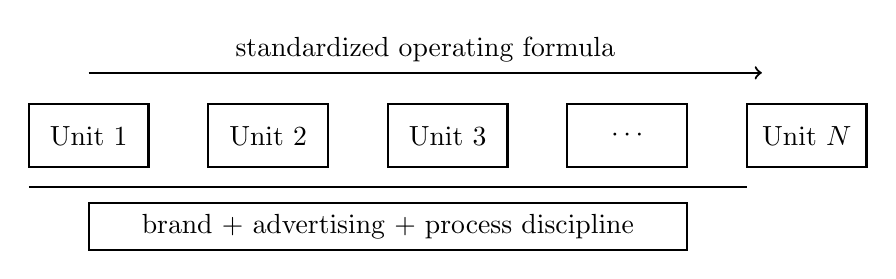
\begin{tikzpicture}[x=1.9cm,y=1cm]
\draw[thick] (0,0) -- (4.8,0);
\foreach \x/\lab in {0/{Unit 1},1.2/{Unit 2},2.4/{Unit 3},3.6/{\(\cdots\)},4.8/{Unit \(N\)}}{
  \draw[thick] (\x,0.25) rectangle (\x+0.8,1.05);
  \node at (\x+0.4,0.65) {\lab};
}
\draw[thick,->] (0.4,1.45) -- (4.9,1.45);
\node at (2.65,1.75) {standardized operating formula};
\draw[thick] (0.4,-0.8) rectangle (4.4,-0.2);
\node at (2.4,-0.5) {brand + advertising + process discipline};
\end{tikzpicture}
\end{figure}

The figure is editorial, but it captures the lecture's mechanism faithfully. Scale is not simply more hustle. It is repeated units under a stable operating formula.

\section{Debt, Overextension, and the Household Constraint}

The next physician is not even at home. He answers remotely from California while the interviewer stands at the Houston property. This is one of the lecture's sharpest pivots. After expansion, the lecture turns to defense.

The advice is simple and serious: do not overextend yourself; live below your means; otherwise bad times will expose expenses that exceed your capacity. The mathematical content is small, but it is exact enough to preserve:
\begin{equation}
E_t + DS_t < Y_t.
\end{equation}
Here \(E_t\) is living expenditure, \(DS_t\) is debt service, and \(Y_t\) is income. The point is not to decorate the page with symbols. The point is to preserve the speaker's structural claim that resilience requires slack.

\subsection{Question \& Answer}

\paragraph{Question.} Why is ``living below your means'' not merely moral advice, but a real financial constraint?

\paragraph{Answer.} Because bad times are periods in which income may fall, opportunities may narrow, or obligations may become heavy precisely when flexibility is needed. If one has
\begin{equation}
Y_t - (E_t + DS_t) > 0,
\end{equation}
then one has a buffer. If instead
\begin{equation}
Y_t - (E_t + DS_t) < 0,
\end{equation}
then every downturn is amplified by fixed commitments. The lecture's phrase ``don't over-leverage yourself'' is just the same statement in more operational language.

We may draw the idea schematically:

\begin{figure}
\centering
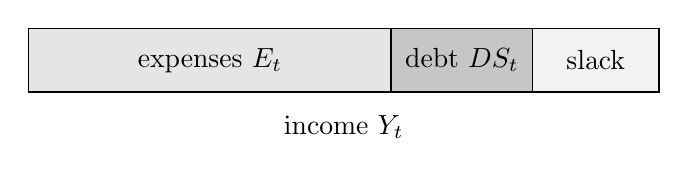
\begin{tikzpicture}[x=1cm,y=1cm]
\draw[thick] (0,0) rectangle (8,0.8);
\draw[fill=gray!20] (0,0) rectangle (4.6,0.8);
\draw[fill=gray!45] (4.6,0) rectangle (6.4,0.8);
\draw[fill=gray!10] (6.4,0) rectangle (8,0.8);
\node at (2.3,0.4) {expenses \(E_t\)};
\node at (5.5,0.4) {debt \(DS_t\)};
\node at (7.2,0.4) {slack};
\node at (4,-0.45) {income \(Y_t\)};
\end{tikzpicture}
\end{figure}

Again, the diagram is editorial. But it is exactly the sort of simple balance-sheet picture the transcript calls for.

\section{Operations, Payroll, and the Rallying Point}

The former auto dealer takes the lecture into a more institutional region. His first important claim is epistemic: school does not really teach operating reality in the form one needs when one begins to run a business. One needs mentorship, instruction, and contact with what the business actually demands under live conditions.

Then the lecture becomes quantitative again. The speaker mentions weekly payroll burdens of
\begin{equation}
B_{\text{week}} \in \{\$150{,}000,\ \$400{,}000,\ \$1{,}000{,}000\}.
\end{equation}
This is the point where the chapter must not be reduced to generic motivation. Payroll is a fixed weekly obligation; it converts entrepreneurship from a private ambition into a public responsibility. Other households depend on the firm's continued functioning.

\subsection{Question \& Answer}

\paragraph{Question.} What changes when success is no longer about your own paycheck, but about making payroll for everyone else?

\paragraph{Answer.} The scale of responsibility changes the internal mathematics of leadership. When payroll is small, one can imagine success as a matter of individual effort. When payroll becomes very large, the problem is organizational. One must coordinate people around a common objective, and that is why the speaker insists on a ``rallying point'' and a motivational focus.

The logic may be written as a sequence:
\begin{enumerate}
\item Weekly payroll \(B_{\text{week}}\) is a fixed claim.
\item As \(B_{\text{week}}\) rises, more families become exposed to business performance.
\item Leadership must therefore become transmissible across a team.
\item A rallying point is needed to align effort.
\item Outwork still matters, but it now matters through organization, not merely through private stamina.
\end{enumerate}

The lecture then resolves the point with a surprisingly austere conclusion: one need not be the smartest, the biggest, or the fastest. One must become the best by outworking everybody else in the organization. This should not be literalized into a precise decomposition of success. But its place in the narrative is exact. The lecture has moved from household discipline to organizational strain, and it resolves the tension through coordinated effort.

\section{Staff, Balance, Capital Formation, and Money as a Tool}

The closing sequence is mosaic-like, but it should not be treated as miscellaneous residue. The chef says that staff are the greatest asset: treat them like gold, and they will respond in kind. This is the labor-side counterpart to the auto dealer's payroll logic. Payroll is the burden; staff quality is the multiplier. In both cases, other people are not secondary to the enterprise. They are the enterprise.

The chef also introduces a balancing clause: work hard, play harder, and do not allow money to erase life itself. One may hear that as soft advice, but within the lecture it functions as a limit on the entire project. Wealth is not only an accumulation problem. It is also an allocation problem across time and experience.

Then the lecture discovers Tillman Fertitta's house and briefly turns the city itself into part of the drama: hidden behind gates are operators, billionaires, and ownership structures one cannot predict from the curb. The point is not celebrity. The point is again epistemic. One does not know, from appearance alone, what mechanism lies behind the house.

The final physician-entrepreneur brings the themes together. He says it took about ten years to understand business. He emphasizes the need to keep learning and to reject the fantasy that success comes easily. He also provides one of the cleanest capital-formation mechanisms in the lecture: during the first year after graduation he worked roughly three times as much as a normal doctor so that he could save enough capital to take to a bank and secure financing for the first facility. In symbolic form, the lecture's logic is
\begin{equation}
\frac{H}{H_{\text{norm}}} \approx 3,
\end{equation}
followed by
\begin{equation}
K_0 = \sum_{t=1}^{T} (Y_t - E_t),
\end{equation}
and then the transition
\begin{equation}
K_0 \text{ sufficient } \Longrightarrow \text{bank loan } L \text{ for the first facility.}
\end{equation}

This is perhaps the cleanest derivation in the latter half of the lecture:
\begin{enumerate}
\item Increase labor input sharply at the beginning.
\item Convert that excess labor into unusually large earned income.
\item Hold consumption down rather than inflating lifestyle.
\item Accumulate initial equity \(K_0\).
\item Use \(K_0\) to unlock external financing \(L\).
\item Build the first facility and begin the entrepreneurial sequence.
\end{enumerate}

The speaker's final financial philosophy is an appropriate closing theorem for the day: do not chase money as the terminal object. Treat money as a tool to do something great. That is not anti-mathematical. It is a statement about objective function. If money is only a symbol of status, then cars and houses become the whole picture. If money is treated as an instrument, then the real variables are projects, ownership, freedom, and durability.

\section{Summary}

The lecture begins with mansions and ends with mechanisms. In between, it offers a sequence of field-tested structures: delayed payoff after migration, compounding through early saving, scale through repeatable systems, freedom through debt reduction, resilience through living below one's means, leadership under payroll pressure, performance through staff quality, and capital formation through early sacrifice.

What makes the lecture worth writing down is precisely that it does not propose a single secret. It proposes a family of quantitative disciplines. We are shown, one doorstep at a time, that visible wealth is usually the surface of something slower and less glamorous: multiplication over time, constraints respected, systems repeated, debts reduced, teams organized, and labor sustained long enough for the arithmetic to turn in one's favor.